In 1828, Jacobi found a beautiful proof for a special case of Poncelet's closure theorem using elliptic functions. In particular, he provided a very simple parametrization for the family of N-sided bicentric polygons that appear in Poncelet's theorem. We will use his parametrization below, and it is appropriate to recall it here.

Referring to Figure~\ref{fig:jacobi-nested}, %and \ref{fig:jacobi-unnested},
consider two circles $\C_{R}$ and $\C_{r}$, with radii $R$ and $r$, respectively. Let $d$ denote the distance between their centers. We will consider polygons that are inscribed in $\C_{R}$ and also are either inscribed or exscribed in $\C_{r}$. By exscribed in $\C_{r}$ we mean that extensions of the sides of the polygon are tangent to $\C_{r}$. Let $p_{j}(u)$, $j=1,...,N$ be the vertices of a N-sided bicentric family of polygons, parametrized by the real variable $u$, with all the vertices in $\C_{R}$.

\begin{figure}
    \centering
  %  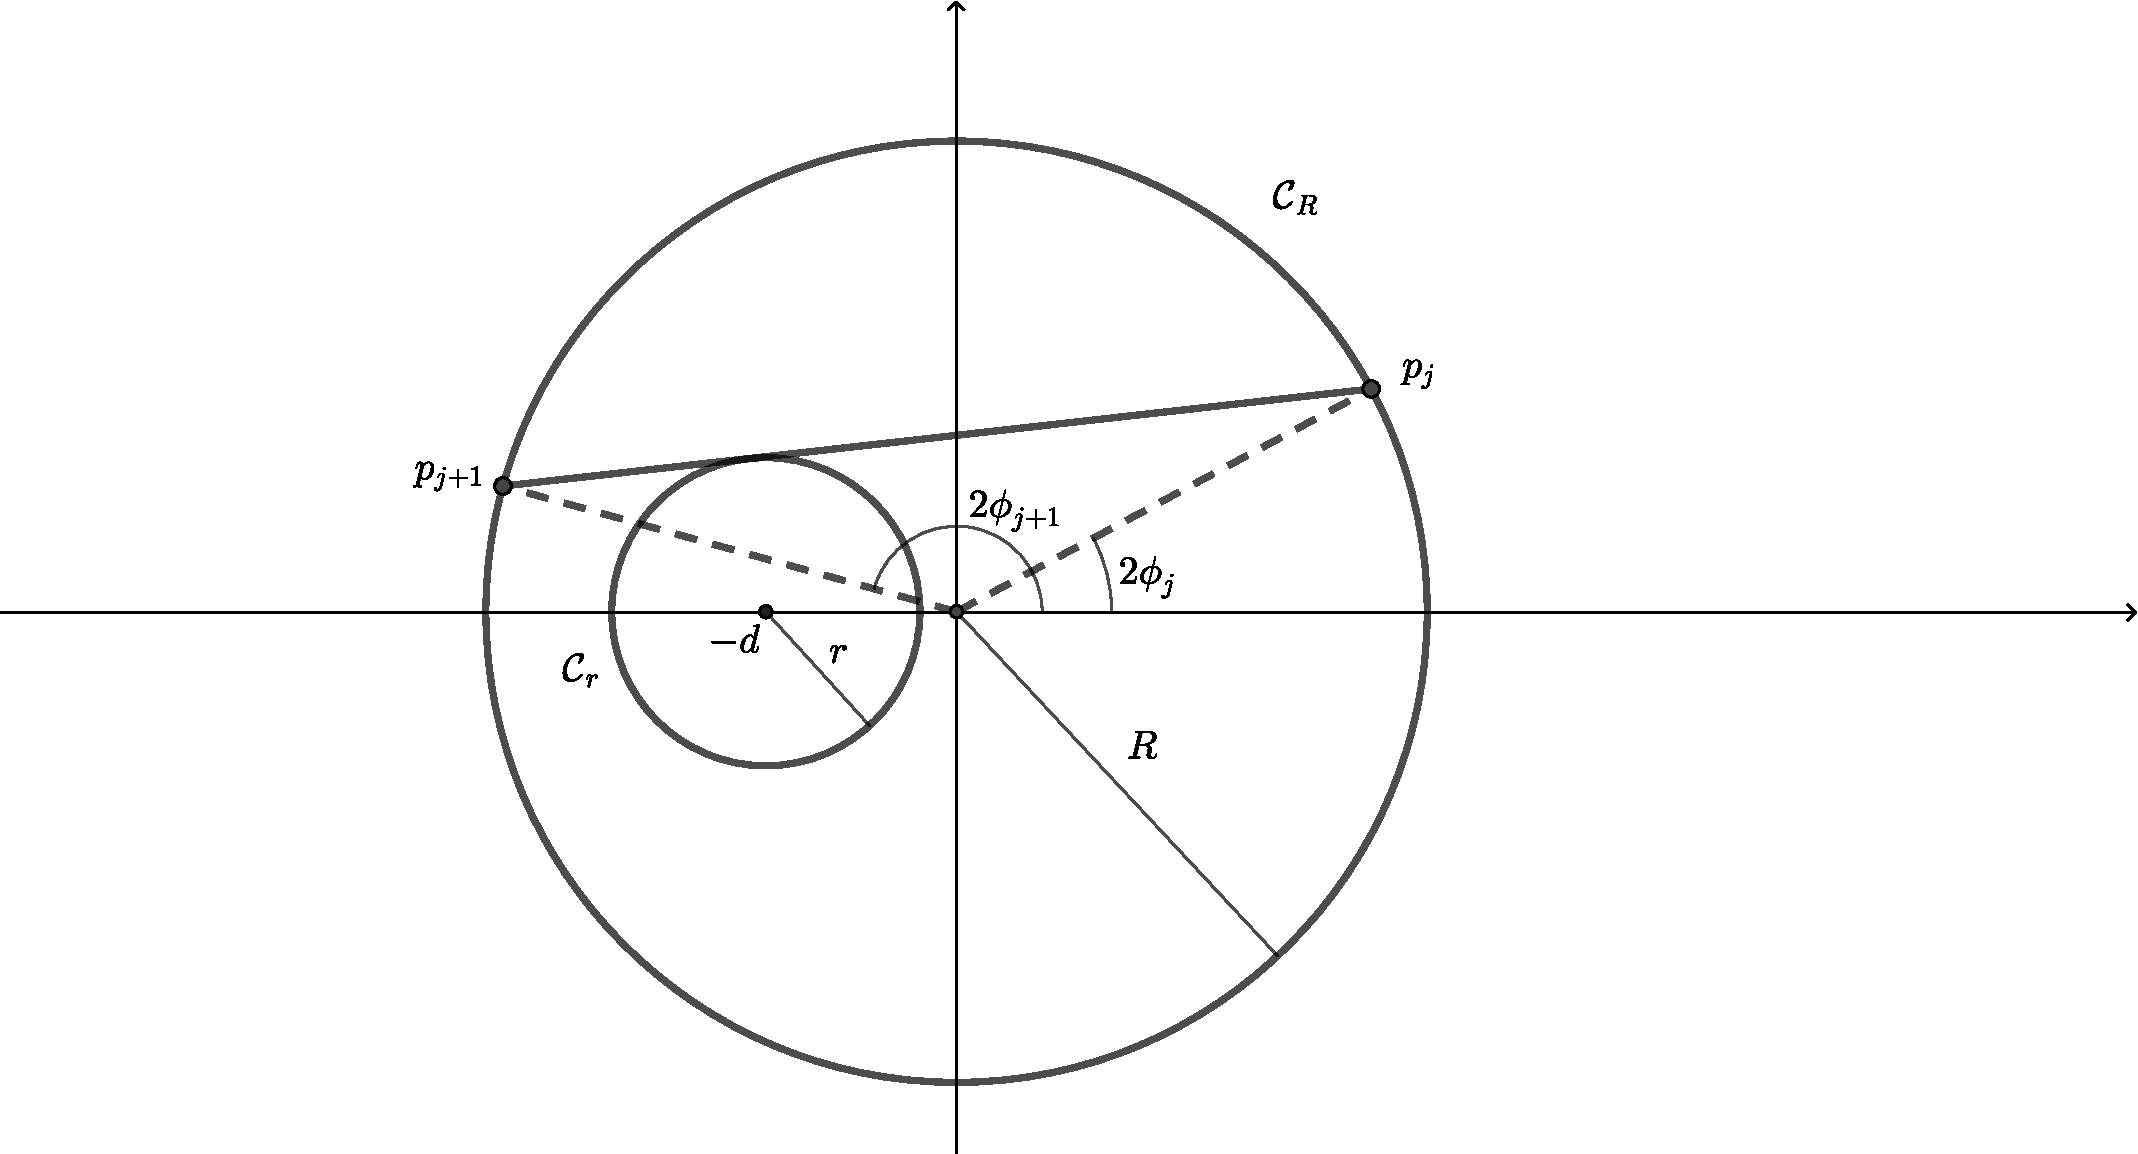
\includegraphics[width=.8\textwidth]{pics_04/0110_inscribed.pdf}
    \caption{A pair of circles, along with a chord $p_j,p_{j+1}$ of the outer circle tangent to the inner one.}
    \label{fig:jacobi-nested}
\end{figure}

%\begin{figure}
%    \centering
%    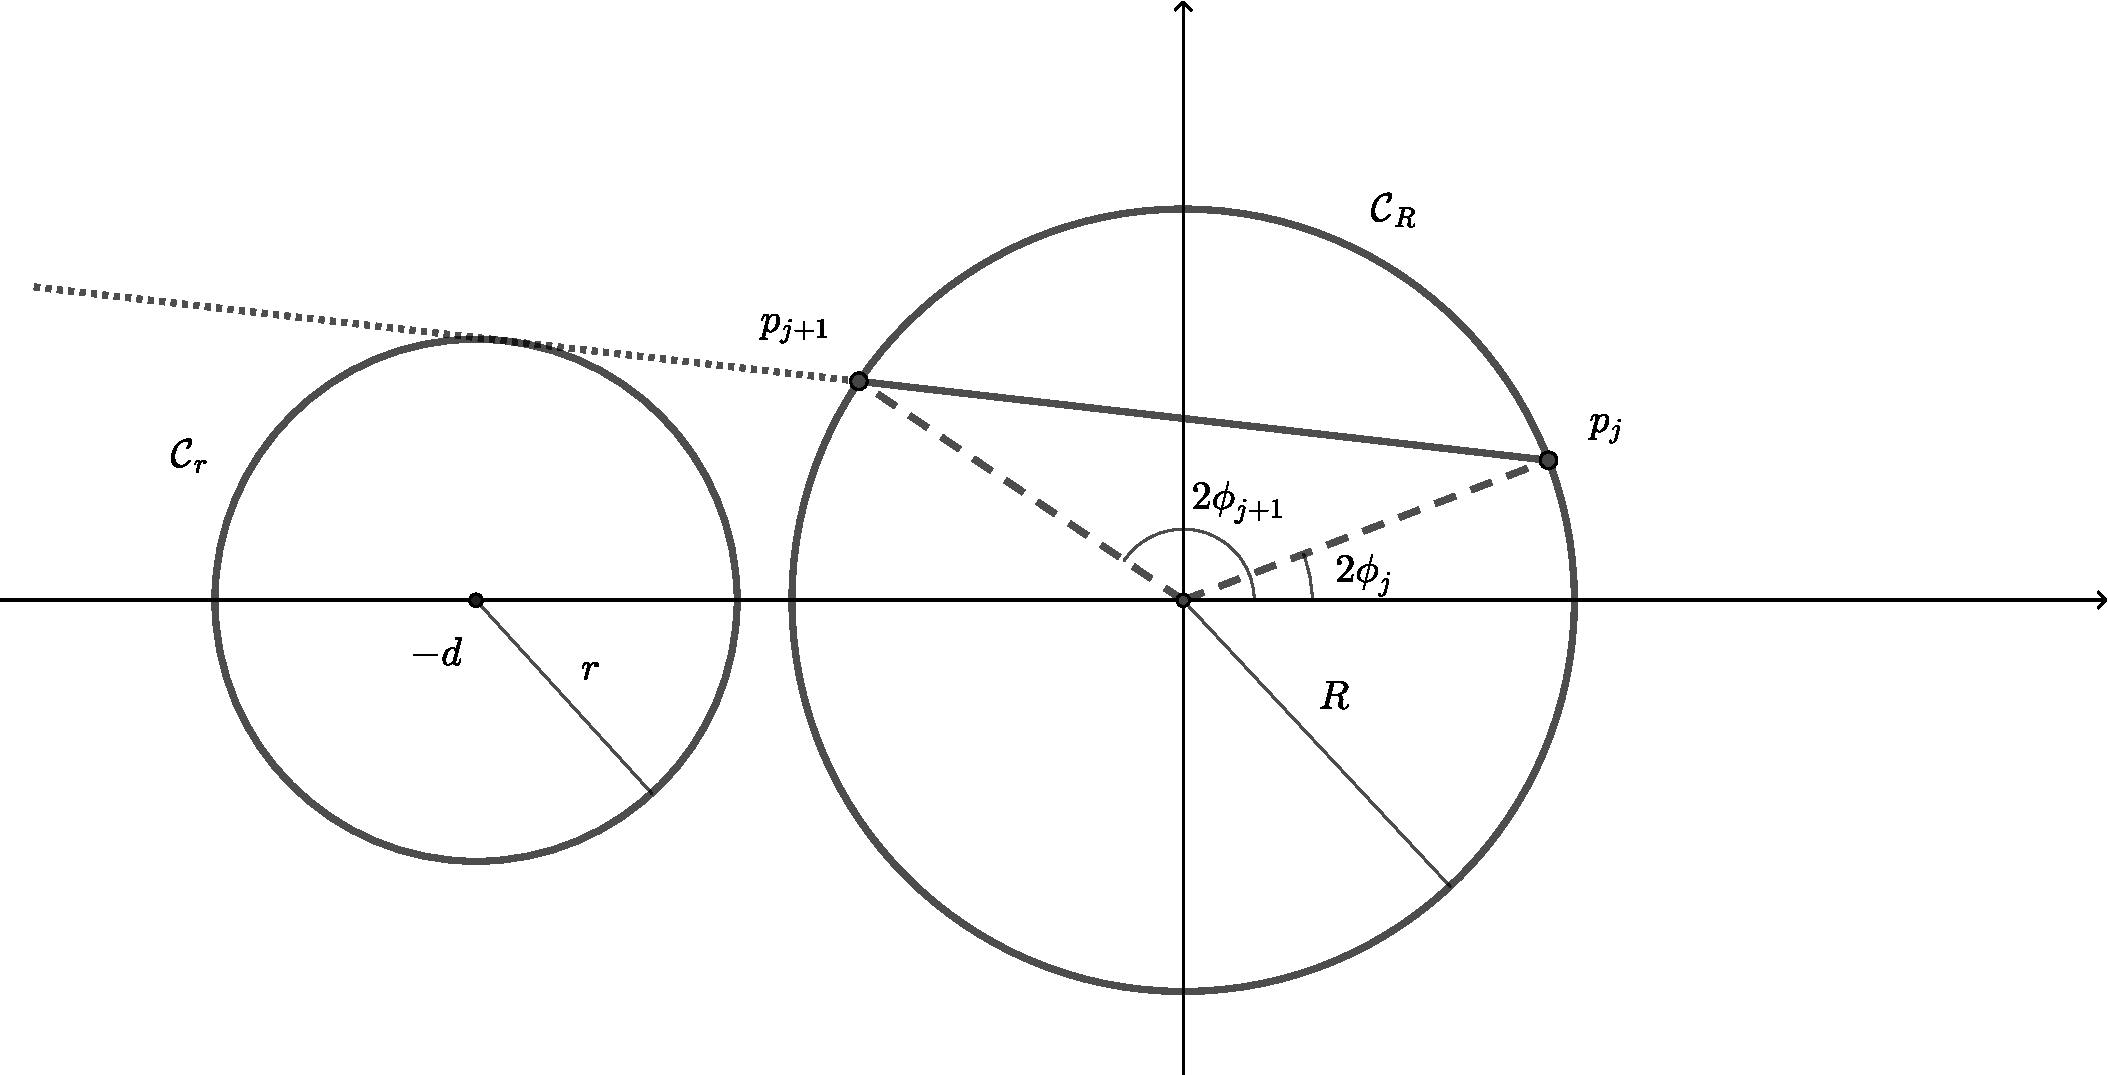
\includegraphics[width=.8\textwidth]{pics/0120_exscribed.pdf}
%    \caption{An unnested bicentric pair $\C_R$, $\C_r$.}
%    \label{fig:jacobi-unnested}
%\end{figure}

Jacobi noticed that his elliptic functions could be used to provide an explicit expression for the $p_{j}(u)$. Namely, if we write
\begin{equation}
\label{jacobivertex}  
p_{j}(u)=R\left[ \cos{(2\phi_{j}(u))}, \sin{(2\phi_{j}(u))}\right]
\end{equation}

Indeed, he proved that \cite{bos-1987}:

\begin{equation}
\label{jacobiangle}
\phi_{j}(u)=am(u+ j \sigma,k),
\end{equation}
%
where $am(u,k)$ is the classical Jacobi amplitude function \cite{armitage-2006}, $k$ is the modulus and it is related to $R$, $r$ and $d$ by the following expression \cite[pp. 315]{bos-1987}:

\begin{equation}
\label{jacobirelation}
k^2=\frac{4Rd}{(R+d)^2-r^2},\;\;\;0<k<1
\end{equation}
 %        
The real number $K$ is defined by:
%
\[K=\int_{0}^{\frac{\pi}{2}} \frac{dt}{\sqrt{1-k^2sin^2{t}}}, \]
and finally, $\sigma$ is given by

\[ \sigma=\frac{4\tau K}{N},\]
where $\tau$ is a positive integer and $N>2$.

Actually, Jacobi treated only the case where one of the circles is inscribed, but his argument also holds for the exscribed case \cite{bos-1987}.

Below we recall some very facts about three of Jacobi's elliptic functions: $sn(z,k)=\sin{(am(z,k))}$, $cn(z,k)=\cos(am(z,k))$ and $dn(z,k)=\sqrt{1-k^2sn^2(z,k)}$, where $z \in \mathbb{C}$, and $0<k<1$ is the elliptic modulus. Since $k$ is fixed, we write $sn(z)$ instead of $sn(z,k)$, etc.

These functions have two independent periods and also have simple poles at the same points. In fact:

\begin{align*}
    sn(u+4K)&=sn(u+2iK')=sn(u)\\
    cn(u+4K)&=cn(u+2K+2iK')=cn(u)\\
    dn(u+2K)&=dn(u+4iK')=dn(u)\\
    K'&=K(k'), \;\;k'=\sqrt{1-k^2}
\end{align*}
The  poles of these three functions, which are simple, occur at the points
\[2mK+i(2n+1)K'
,\;\; m,n\in \mathbb{Z}\]

They also display a certain symmetry around the poles. Namely, if $z_p$ is a pole of $sn(z)$, $cn(z)$ and $dn(z)$, then, for every $w \in \mathbb{C}$, we have \cite[Chapter 2]{armitage-2006}:

\begin{align}
sn(z_p+w)=&-sn(z_p-w) \nonumber \\
cn(z_p+w)=&-cn(z_p-w)  \label{eqn:zpole} \\
dn(z_p+w)=&-dn(z_p-w) \nonumber
\end{align}

 